\documentclass[12pt,a4paper]{article}
\usepackage[utf8]{inputenc}
\usepackage[T2A]{fontenc}
\usepackage[russian]{babel}
\usepackage{amsmath,amssymb}
\usepackage{geometry}
\usepackage{graphicx}
\usepackage{hyperref}
\geometry{margin=2.2cm}

\title{Лабораторная работа: численные методы вычисления интегралов\\[4pt]
\large Вариант 1: $f(x)=x^2$, $[a,b]=[1,2]$}
\author{Трикашный М.\,Д.}
\date{}

\begin{document}
\maketitle

\section*{Часть 1. Интегральные суммы и численное интегрирование}

\subsection*{1. Интегральная сумма}

Разбиение отрезка $[1,2]$ равномерное: $x_k = 1 + \dfrac{k}{n}$, $k=0,\dots,n$,
$\Delta x_k = \dfrac{1}{n}$. Возьмём для определённости \emph{левое}
оснащение, $\xi_i = x_{i-1}$. Тогда интегральная сумма Римана имеет вид
\[
  \sigma_n \;=\; \sum_{i=1}^{n} f(\xi_i)\,\Delta x_i
  \;=\; \frac{1}{n}\sum_{i=1}^{n}\Bigl(1+\tfrac{i-1}{n}\Bigr)^{\!2}.
\]

\subsection*{2. Предел интегральных сумм}

Раскроем квадрат:
\[
  \sigma_n
  = \frac{1}{n}\sum_{i=1}^{n}\!\left(1+\frac{2(i-1)}{n}+\frac{(i-1)^2}{n^2}\right)
  = 1 + \frac{2}{n^2}\sum_{i=1}^{n}(i-1) + \frac{1}{n^3}\sum_{i=1}^{n}(i-1)^2.
\]
Используя $\sum_{k=0}^{n-1}k=\dfrac{n(n-1)}{2}$ и
$\sum_{k=0}^{n-1}k^2=\dfrac{(n-1)n(2n-1)}{6}$, получим
\[
  \sigma_n = 1 + \frac{n-1}{n} + \frac{(n-1)(2n-1)}{6n^2}
  \;\xrightarrow[n\to\infty]{}\; 1+1+\frac{2}{6} = \frac{7}{3}.
\]

\subsection*{3. Существование интеграла Римана}

Функция $f(x)=x^2$ непрерывна на отрезке $[1,2]$, следовательно она
интегрируема по Риману (теорема о интегрируемости непрерывной функции на
компакте). Этого достаточно. Альтернативное доказательство через
критерий Дарбу: $f$ монотонно возрастает на $[1,2]$, поэтому на каждом
$[x_{i-1},x_i]$ выполнено $m_i=f(x_{i-1})$, $M_i=f(x_i)$ и
\[
  S_n - s_n
  = \sum_{i=1}^{n}\bigl(f(x_i)-f(x_{i-1})\bigr)\Delta x
  = \Delta x\,\bigl(f(b)-f(a)\bigr) = \frac{f(2)-f(1)}{n} = \frac{3}{n}\to 0.
\]

\subsection*{4. Проверка по формуле Ньютона--Лейбница}

\[
  \int_{1}^{2} x^2\,dx = \left.\frac{x^3}{3}\right|_{1}^{2}
  = \frac{8}{3}-\frac{1}{3} = \frac{7}{3} \approx 2{,}33333\ldots
\]
Совпадает с пределом из п.~2.

\subsection*{5--6. Программа и сравнение с теорией}

Программа \texttt{integral\_sums.py} реализует четыре способа: левые,
правые, средние прямоугольники и формулу трапеций; рисует ступенчатую
фигуру и выводит значение суммы. Запуск:
\begin{verbatim}
python integral_sums.py -n 10 --save-dir screenshots
python integral_sums.py -n 100 --save-dir screenshots
\end{verbatim}

\paragraph{Таблица результатов.} Точное значение $I=7/3\approx 2{,}3333333$.

\begin{center}
\begin{tabular}{l|rrr|rrr}
       & \multicolumn{3}{c|}{$n=10$} & \multicolumn{3}{c}{$n=100$}\\
метод  & $\sigma_n$ & $|\Delta|$ & теор.\ оценка
       & $\sigma_n$ & $|\Delta|$ & теор.\ оценка \\\hline
левые     & $2{,}18500$ & $1{,}48\!\cdot\!10^{-1}$ & $2{,}0\!\cdot\!10^{-1}$
          & $2{,}31835$ & $1{,}50\!\cdot\!10^{-2}$ & $2{,}0\!\cdot\!10^{-2}$\\
правые    & $2{,}48500$ & $1{,}52\!\cdot\!10^{-1}$ & $2{,}0\!\cdot\!10^{-1}$
          & $2{,}34835$ & $1{,}50\!\cdot\!10^{-2}$ & $2{,}0\!\cdot\!10^{-2}$\\
средние   & $2{,}33250$ & $8{,}33\!\cdot\!10^{-4}$ & $8{,}33\!\cdot\!10^{-4}$
          & $2{,}333325$& $8{,}33\!\cdot\!10^{-6}$ & $8{,}33\!\cdot\!10^{-6}$\\
трапеции  & $2{,}33500$ & $1{,}67\!\cdot\!10^{-3}$ & $1{,}67\!\cdot\!10^{-3}$
          & $2{,}33335$ & $1{,}67\!\cdot\!10^{-5}$ & $1{,}67\!\cdot\!10^{-5}$\\
\end{tabular}
\end{center}

Видно, что фактические погрешности \emph{не превосходят} теоретических
оценок (а для средних прямоугольников и трапеций фактически совпадают с
теоретической верхней границей --- это потому, что $f''=2=\mathrm{const}$,
и в выводе оценки нет «запаса» из-за переменности второй производной).
При $n\to10n$ погрешность прямоугольников падает в $\sim 10$ раз
($O(1/n)$), а средних и трапеций --- в $\sim 100$ раз ($O(1/n^2)$).

\subsection*{Скриншоты}

\begin{center}
\includegraphics[width=0.48\linewidth]{screenshots/n10_left.png}
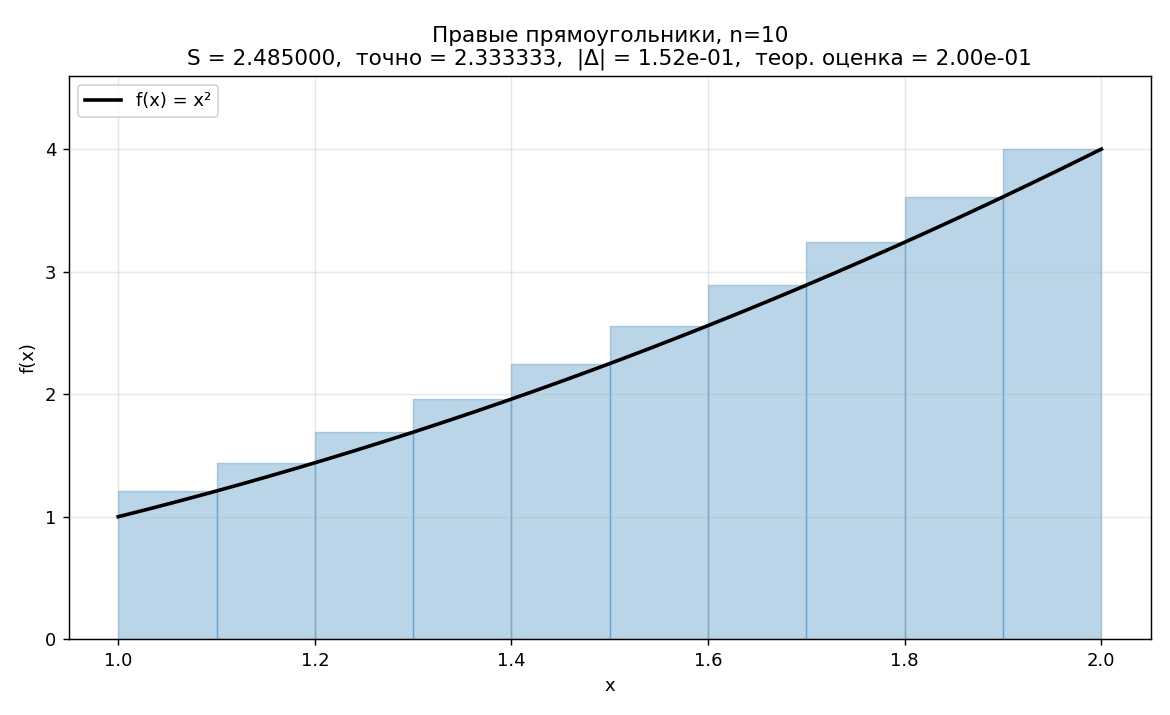
\includegraphics[width=0.48\linewidth]{screenshots/n10_right.png}\\[3pt]
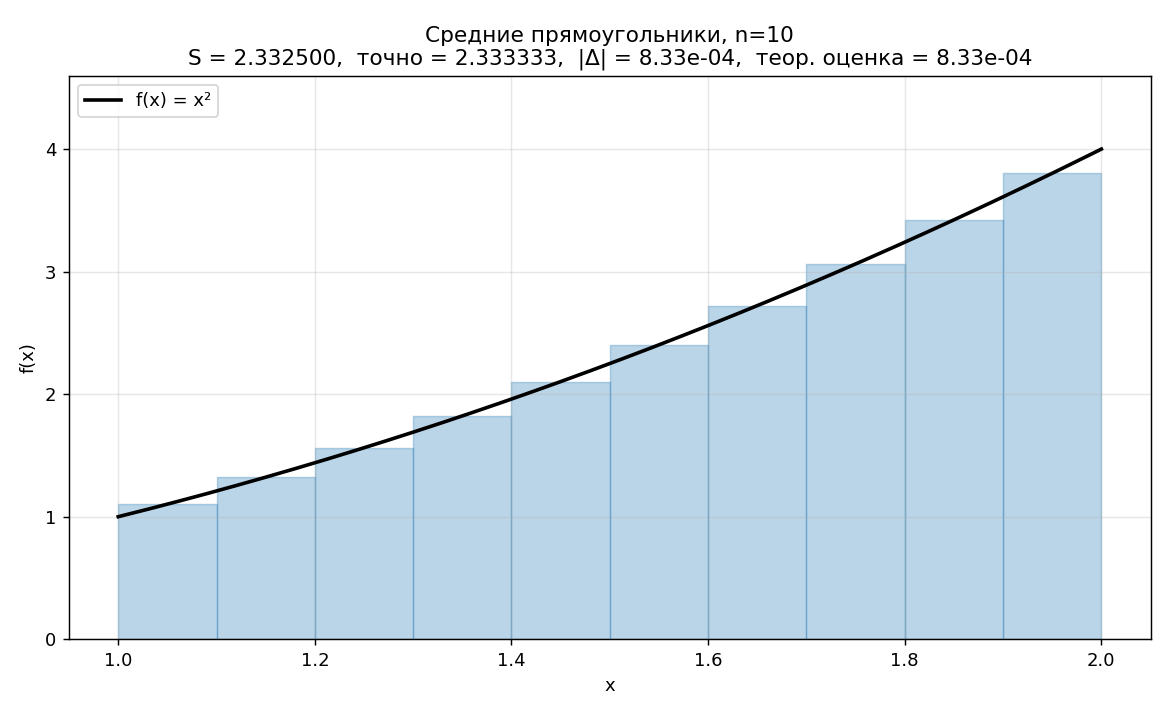
\includegraphics[width=0.48\linewidth]{screenshots/n10_mid.png}
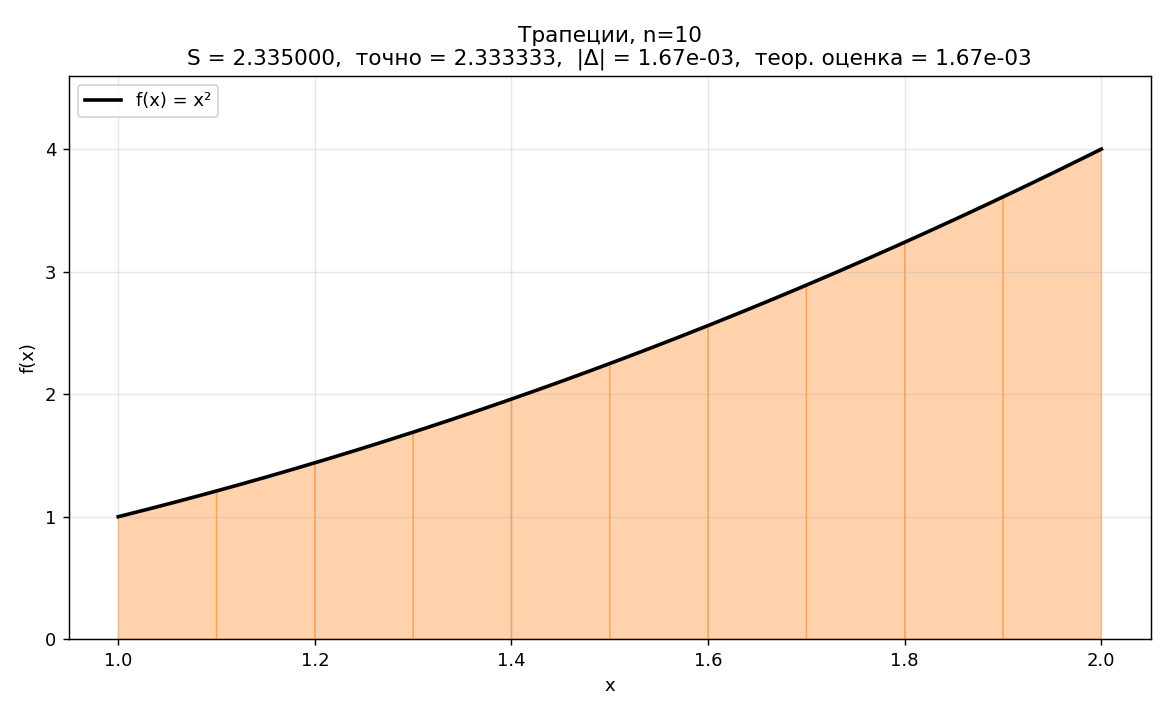
\includegraphics[width=0.48\linewidth]{screenshots/n10_trap.png}\\[3pt]
\small Интегральные суммы при $n=10$ (левые, правые, средние, трапеции).
\end{center}

\begin{center}
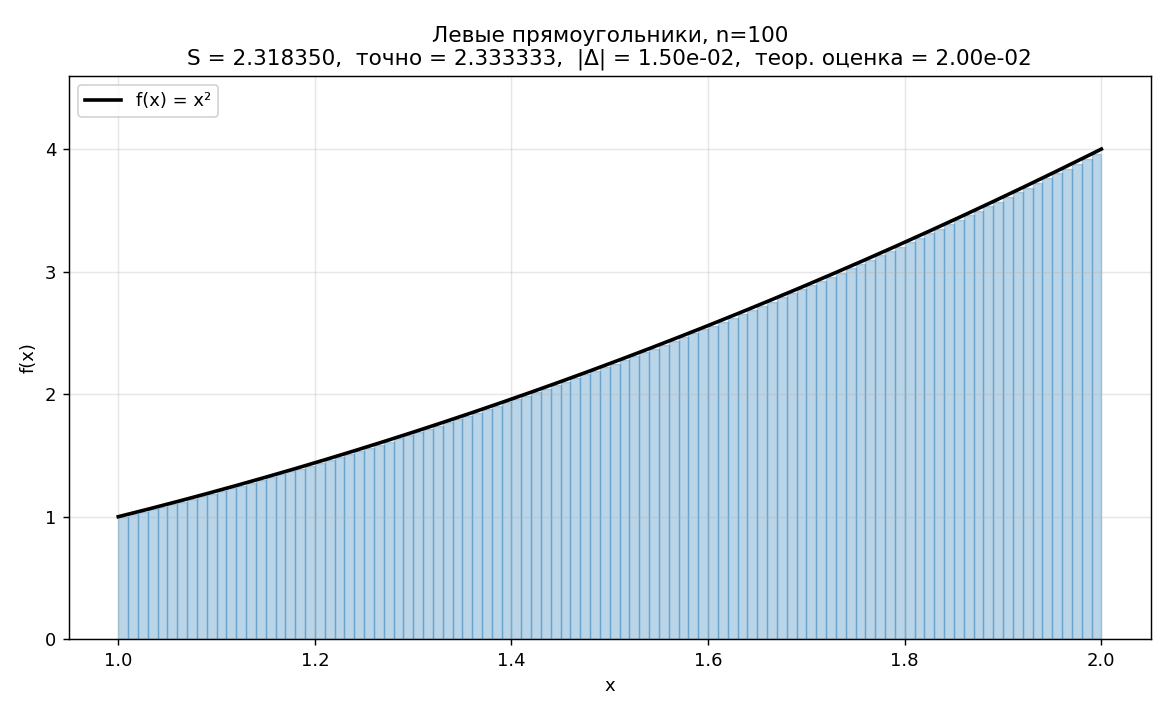
\includegraphics[width=0.48\linewidth]{screenshots/n100_left.png}
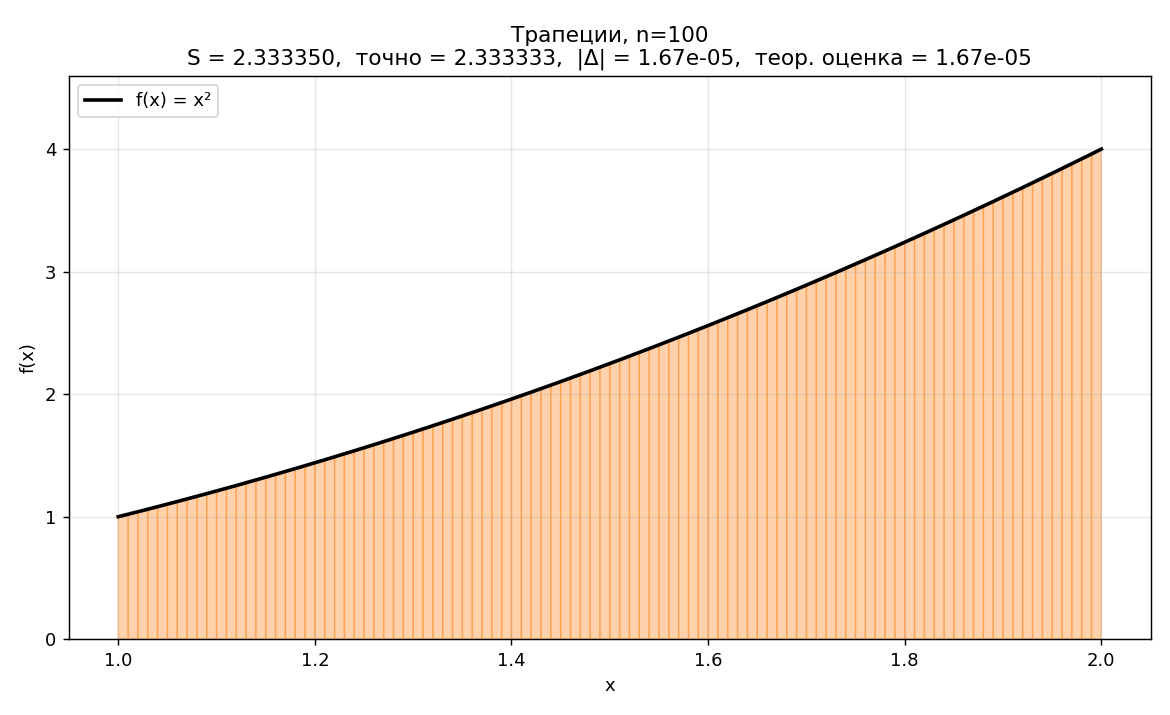
\includegraphics[width=0.48\linewidth]{screenshots/n100_trap.png}\\
\small То же при $n=100$ (левые и трапеции).
\end{center}

\subsection*{7. Вывод формул для погрешности}

Пусть $\Delta x = (b-a)/n$, $\Delta_i=[x_{i-1},x_i]$.

\paragraph{Левые/правые прямоугольники ($f\in C^1[a,b]$).} По формуле
Тейлора с остатком в форме Лагранжа:
$f(x)=f(x_{i-1})+f'(\xi)(x-x_{i-1})$, $\xi\in(x_{i-1},x)$. Тогда
\[
  \int_{x_{i-1}}^{x_i}\!\!f\,dx - f(x_{i-1})\Delta x
  = \int_{x_{i-1}}^{x_i}\!\!f'(\xi)(x-x_{i-1})\,dx,
\]
\[
  \left|\int_{x_{i-1}}^{x_i}\!\!f\,dx - f(x_{i-1})\Delta x\right|
  \le \max_{\Delta_i}|f'|\int_{x_{i-1}}^{x_i}(x-x_{i-1})\,dx
  = \tfrac{1}{2}\max_{\Delta_i}|f'|\,\Delta x^2.
\]
Суммируя:
\[
  |R_n|\le \tfrac{1}{2}n\Delta x^2\max_{[a,b]}|f'|
  = \frac{(b-a)^2}{2n}\max_{[a,b]}|f'(x)|.
\]
Для правых прямоугольников вывод аналогичен.

\paragraph{Средние прямоугольники ($f\in C^2[a,b]$).}
Раскладывая в ряд Тейлора в середине $c_i=\tfrac{x_{i-1}+x_i}{2}$:
$f(x)=f(c_i)+f'(c_i)(x-c_i)+\tfrac{1}{2}f''(\eta)(x-c_i)^2$. Интеграл от
линейного члена по симметричному отрезку равен нулю, поэтому
\[
  \int_{x_{i-1}}^{x_i}\!\!f\,dx - f(c_i)\Delta x
  = \tfrac{1}{2}\!\int_{x_{i-1}}^{x_i}\!\!f''(\eta)(x-c_i)^2\,dx,
\]
\[
  \Bigl|\,\cdot\,\Bigr|
  \le \tfrac{1}{2}\max_{\Delta_i}|f''|\cdot 2\!\int_0^{\Delta x/2}\!\!t^2\,dt
  = \frac{\Delta x^3}{24}\max_{\Delta_i}|f''|.
\]
Суммируя по всем $n$ отрезкам:
\[
  |R_n|\le \frac{n\Delta x^3}{24}\max_{[a,b]}|f''|
  = \frac{(b-a)^3}{24n^2}\max_{[a,b]}|f''(x)|.
\]

\paragraph{Трапеции ($f\in C^2[a,b]$).} На каждом $\Delta_i$ заменим $f$
линейным интерполянтом $L_i$ по узлам $x_{i-1},x_i$. Погрешность
интерполяции:
$f(x)-L_i(x)=\tfrac{1}{2}f''(\eta)(x-x_{i-1})(x-x_i)$. Тогда
\[
  \int_{x_{i-1}}^{x_i}\!(f-L_i)\,dx
  = \tfrac{1}{2}\!\int_{x_{i-1}}^{x_i}\!f''(\eta)(x-x_{i-1})(x-x_i)\,dx,
\]
\[
  \left|\cdot\right|
  \le \tfrac{1}{2}\max_{\Delta_i}|f''|\!\int_{x_{i-1}}^{x_i}\!(x-x_{i-1})(x_i-x)\,dx
  = \tfrac{1}{2}\max_{\Delta_i}|f''|\cdot \tfrac{\Delta x^3}{6}
  = \frac{\Delta x^3}{12}\max_{\Delta_i}|f''|.
\]
Суммируя:
\[
  |R_n|\le \frac{(b-a)^3}{12n^2}\max_{[a,b]}|f''(x)|.
\]

\paragraph{Применение к варианту 1.} $f(x)=x^2$, $[1,2]$,
$f'(x)=2x$, $\max|f'|=4$; $f''(x)=2$, $\max|f''|=2$; $b-a=1$. Подстановка:
\begin{align*}
\text{лев./прав.:}\quad & |R_n|\le \frac{4\cdot 1}{2n}=\frac{2}{n},\\
\text{средние:}\quad    & |R_n|\le \frac{2\cdot 1}{24n^2}=\frac{1}{12n^2},\\
\text{трапеции:}\quad   & |R_n|\le \frac{2\cdot 1}{12n^2}=\frac{1}{6n^2}.
\end{align*}
При $n=10$: $2/n=0{,}2$; $1/(12n^2)\approx 8{,}33\!\cdot\!10^{-4}$;
$1/(6n^2)\approx 1{,}67\!\cdot\!10^{-3}$ --- ровно то, что в таблице.

\section*{Часть 2. Маятник}

\textbf{Замечание.} Эта часть требует постановки физического эксперимента
с реальным маятником (длинная нить, тяжёлый груз) и видеосъёмки
колебаний для нескольких углов. Здесь приводятся аналитические пункты;
видео и обработка движения по кадрам выполняются отдельно.

\subsection*{Малые колебания: вывод формулы (3)}

Уравнение $\theta''+\omega^2\theta=0$ с $\theta(0)=\theta_0$,
$\theta'(0)=0$. Домножая на $\theta'$ и интегрируя по $[0,t]$, получаем
$\theta'^2+\omega^2(\theta^2-\theta_0^2)=0$, откуда
$d\theta/\sqrt{\theta_0^2-\theta^2}=\pm\omega\,dt$. Интегрирование даёт
$\arcsin(\theta/\theta_0)-\pi/2=\pm\omega t$, то есть
$\theta(t)=\theta_0\cos(\omega t)$. Период $T=2\pi/\omega=2\pi\sqrt{L/g}$.
Переход $\sin\theta\approx\theta$ оправдан тем, что
$\sin\theta=\theta-\theta^3/6+O(\theta^5)$, поэтому относительная ошибка
замены порядка $\theta_0^2/6$; при $\theta_0<10^\circ\approx0{,}175$
рад это $<0{,}5\%$.

\subsection*{Нелинейная модель: доказательство формулы (6)}

В интеграле
$\displaystyle\int_0^{\theta_0}\!\frac{d\theta}{\sqrt{\cos\theta-\cos\theta_0}}$
воспользуемся тождеством $\cos\theta=1-2\sin^2(\theta/2)$:
\[
  \cos\theta-\cos\theta_0
  = 2\bigl(\sin^2(\theta_0/2)-\sin^2(\theta/2)\bigr).
\]
Введём замену $\sin(\theta/2)=\sin(\theta_0/2)\sin u =: k\sin u$, где
$k=\sin(\theta_0/2)$. Тогда
$\tfrac{1}{2}\cos(\theta/2)\,d\theta = k\cos u\,du$ и
\[
  d\theta = \frac{2k\cos u\,du}{\cos(\theta/2)}
         = \frac{2k\cos u\,du}{\sqrt{1-k^2\sin^2 u}}.
\]
Под корнем:
$\sqrt{\cos\theta-\cos\theta_0}=\sqrt{2}\sqrt{k^2-k^2\sin^2 u}
= k\sqrt{2}\cos u$. Пределы: $\theta=0\Rightarrow u=0$;
$\theta=\theta_0\Rightarrow \sin u=1\Rightarrow u=\pi/2$. Получаем
\[
  \int_0^{\theta_0}\!\frac{d\theta}{\sqrt{\cos\theta-\cos\theta_0}}
  = \int_0^{\pi/2}\!\frac{2k\cos u}{k\sqrt{2}\cos u}\cdot
    \frac{du}{\sqrt{1-k^2\sin^2 u}}
  = \sqrt{2}\int_0^{\pi/2}\!\frac{du}{\sqrt{1-k^2\sin^2 u}}
  = \sqrt{2}\,F\!\left(\tfrac{\pi}{2},k\right).
\]
\textit{Замечание.} В методичке формула~(6) записана как
$F(\pi/2,\sin(\theta_0/2))$ без множителя $\sqrt2$; этот множитель
поглощается в формулу~(5) (см.\ коэффициент $2\sqrt2/\omega$): с учётом
доказанного равенства $T=\tfrac{4}{\omega}K(k)$, где $K(k)=F(\pi/2,k)$ ---
полный эллиптический интеграл первого рода.

\subsection*{Период по ряду (7)}

\[
  K(k)=\frac{\pi}{2}\sum_{n=0}^{\infty}\!\left(\frac{(2n-1)!!}{(2n)!!}\,k^{n}\right)^{\!2}.
\]
\emph{Замечание.} В печати формулы есть опечатка: правильно стоит $k^n$, но
обычное разложение --- $k^{2n}$. Используем стандартное:
$K(k)=\frac{\pi}{2}\Bigl(1+\bigl(\tfrac12\bigr)^2 k^2
+\bigl(\tfrac{1\cdot3}{2\cdot4}\bigr)^2 k^4+\dots\Bigr)$.
Тогда $T=\tfrac{4}{\omega}K(k)=T_0\cdot\tfrac{2}{\pi}K(k)$ с
$T_0=2\pi\sqrt{L/g}$. Для $\theta_0=30^\circ$, $k=\sin15^\circ\approx0{,}2588$:
\begin{itemize}
  \item 1 слагаемое: $T\approx T_0$ --- относит.\ ошибка $\sim k^2/4\approx1{,}7\%$;
  \item 2 слагаемых: $T\approx T_0(1+k^2/4)\approx 1{,}01675\,T_0$;
  \item 3 слагаемых: $T\approx T_0\bigl(1+k^2/4+9k^4/64\bigr)
        \approx 1{,}01738\,T_0$.
\end{itemize}
С ростом $\theta_0$ роль высших слагаемых растёт; при $\theta_0\to\pi$
ряд сходится крайне медленно, поскольку $k\to 1$.

\subsection*{Что требуется снять и обработать (для отчёта по эксперименту)}

\begin{enumerate}
  \item Малые колебания: для $\theta_0\le 10^\circ$ построить
  $\theta(t)$ по кадрам видео, сравнить с $\theta_0\cos\omega t$;
  измерить период секундомером по 10--20 колебаниям и сравнить с
  $T_0=2\pi\sqrt{L/g}$.
  \item Большие колебания: $\theta_0=30^\circ,45^\circ,60^\circ$, измерить
  период; теоретический период вычислить (а) численно по~(5)
  ранее запрограммированными методами (формула трапеций даёт ошибку
  $\sim 1/n^2$), (б) через ряд из 1/2/3 слагаемых.
  \item Источники погрешности: измерение $L$ (рулетка $\pm 1$\,мм),
  начального угла ($\pm 1^\circ$), периода ($\pm 0{,}05$\,с при
  стартстопе секундомером, на порядок меньше при покадровом анализе),
  затухание (сопротивление воздуха, трение в подвесе).
\end{enumerate}

\end{document}
